\documentclass[11pt,letterpaper]{article}
\usepackage[margin=1in]{geometry}
\usepackage{booktabs}
\usepackage{graphicx}
\graphicspath{{sweep_results/plots/}}
\usepackage{amsmath}
\usepackage{hyperref}
\usepackage{float}
\usepackage{caption}
\usepackage{subcaption}
\usepackage{parskip}
\setlength{\parskip}{6pt}

\title{\textbf{Sequential Prefetching with a Stream Buffer:\\
Implementation and Empirical Evaluation}}
\author{Aengus McGuinness, Ali Saffrini, Madison Gates, Jacob Tom}
\date{}

\begin{document}
\maketitle

%─────────────────────────────────────────────────────────────────────────────
\section*{Abstract}
%─────────────────────────────────────────────────────────────────────────────

This report presents an implementation and empirical evaluation of Jouppi's
stream buffer prefetcher~\cite{jouppi1990improving} within a Pin-based cache
hierarchy simulator. The stream buffer is modeled as a set of independent
FIFO queues sitting between the L1 data cache and L2. On an L1D miss the
simulator checks whether the missed block resides at the head of any active
stream; a hit pops the head and prefetches the next tail line, keeping the
buffer perpetually full. A miss allocates a new sequential stream beginning
one block past the faulting address. The design is evaluated against three
SPEC CPU2006 workloads---\texttt{libquantum}, \texttt{hmmer}, and
\texttt{dealII}---across a sweep of buffer depths (0--8 lines), stream counts
(1--16), and L1D associativities (1--8-way). Results confirm the theoretical
prediction that the prefetcher is highly beneficial for purely sequential
workloads, harmful in terms of L2 bandwidth for irregular workloads, and
marginally effective for mixed-access workloads.

% %─────────────────────────────────────────────────────────────────────────────
% \section{Introduction}
% %─────────────────────────────────────────────────────────────────────────────

% Processor performance is increasingly limited by the latency gap between the
% L1 data cache and main memory. One classical response to this gap is
% prefetching: issuing memory requests before the demand access occurs so the
% data arrives in time. Jouppi's 1990 paper introduced the stream buffer as a
% simple, hardware-efficient prefetch mechanism that works without requiring
% program modification or compiler support.

% The core insight is that many cache misses arise from sequential traversals of
% large arrays that do not fit in the L1 cache. A stream buffer monitors the
% miss stream and, upon detecting a new miss, immediately begins fetching the
% next \(D\) consecutive cache blocks into a FIFO queue. If the next demand
% access hits the head of the queue, the line is delivered at near-L1 speed, the
% queue advances, and a new tail block is fetched to maintain depth. Because the
% queue operates as a separate structure rather than polluting the L1 cache, it
% does not disturb the working set currently resident there.

% This implementation extends that idea to support \(N\) independent streams,
% allowing the prefetcher to track multiple concurrent sequential traversals
% simultaneously. The simulator is built as an Intel Pin tool and measures
% effective L1D misses (demand misses not satisfied by the stream buffer) and
% total L2 requests (demand plus prefetch traffic) over five billion retired
% instructions per benchmark.

%─────────────────────────────────────────────────────────────────────────────
\section{Implementation}
%─────────────────────────────────────────────────────────────────────────────

\subsection{Cache Hierarchy}

The simulator models a three-level hierarchy: an L1 instruction cache, an L1
data cache, an L2 unified cache, and a memory object that counts main-memory
accesses. Each level is derived from a common \texttt{cache} base class that
implements LRU replacement, tag/set extraction, and hit/miss accounting. Cache
parameters (block size, total size, associativity) are read from a
configuration file at startup.

The L1D (\texttt{l1dcache}) overrides the standard \texttt{addressRequest}
method to insert the stream buffer into the miss path. On every L1D miss the
simulator first queries the stream buffer; only on a combined miss does it fall
through to L2 and allocate a new stream.

\subsection{Stream Buffer Data Structure}

The stream buffer is implemented in the \texttt{stream\_buf} class. Its state
consists of an array of \(N\) stream descriptors, each holding a validity flag
and a \texttt{head} field---the block-aligned address of the oldest prefetched
line currently in that stream's FIFO:

\begin{verbatim}
struct Stream {
    bool          valid;
    unsigned long head;
};
\end{verbatim}

The depth \(D\) is not stored explicitly per stream entry; instead, the
invariant is that when a stream is valid, blocks \texttt{[head, head + D*B)}
have already been issued to L2 as prefetches, where \(B\) is the block size.

\subsection{Access Protocol}

When \texttt{l1dcache::addressRequest} records an L1D miss it calls
\texttt{stream\_buf::access(address)}. The method scans all \(N\) stream
descriptors for a head match:

\begin{verbatim}
for( int i = 0; i < nStreams; i++ ) {
    if( !streams[i].valid || streams[i].head != blockAddr )
        continue;

    hits++;
    unsigned long newTailAddr =
        streams[i].head + (unsigned long)depth * blockSz;
    streams[i].head += blockSz;
    if( nextLevel != nullptr )
        nextLevel->addressRequest(newTailAddr);
    return true;
}
return false;
\end{verbatim}

On a stream-buffer hit, the head advances by one block and a single new tail
request is issued to L2. This keeps the buffer perpetually \(D\) lines deep
without re-issuing the lines that are still valid ahead of the head.

\subsection{Allocation Protocol}

On a combined L1D and stream-buffer miss, \texttt{allocate\_stream} is called.
It selects a stream slot---preferring an unused (invalid) slot and falling back
to round-robin eviction---and issues \(D\) consecutive prefetch requests to L2
starting one block past the faulting address:

\begin{verbatim}
unsigned long startAddr = blockAddr + blockSz;
for( int i = 0; i < depth; i++ )
    nextLevel->addressRequest(
        startAddr + (unsigned long)i * blockSz);
streams[idx].valid = true;
streams[idx].head  = startAddr;
\end{verbatim}

The faulting line itself is fetched by the L1D miss handler; the stream buffer
begins one block \emph{ahead} of it, matching Jouppi's original design.

\subsection{L1D Miss Path}

The complete L1D miss path is:
\begin{enumerate}
    \item Record the miss; identify the LRU eviction candidate.
    \item Query \texttt{stream\_buf::access(address)}.
    \item If hit: the line is delivered; L1D is filled. No L2 demand fetch.
    \item If miss: issue a demand fetch to L2; call
          \texttt{allocate\_stream(address)}.
    \item In both cases, install the new line at the LRU slot and update LRU
          metadata.
\end{enumerate}

%─────────────────────────────────────────────────────────────────────────────
\section{Experimental Methodology}
%─────────────────────────────────────────────────────────────────────────────

All experiments use a fixed base configuration: a 64-byte block, 32\,KB
8-way L1I, and a 512\,KB 8-way L2. Experiments vary the L1D configuration.
Simulations are capped at five billion retired instructions per run, executed
under Intel Pin with 102 total configurations spread across four sweeps:

\begin{itemize}
    \item \textbf{Associativity sweep.} L1D varies over 1, 2, 4, 8-way with
          no stream buffer. Isolates conflict-miss behavior from prefetch
          effects.
    \item \textbf{Depth sweep.} Direct-mapped L1D, one stream, depth $D \in
          \{0,1,2,4,8\}$.
    \item \textbf{Stream-count sweep.} Direct-mapped L1D, depth = 1, streams
          $N \in \{1,2,4,8,16\}$.
    \item \textbf{2D sweep.} Direct-mapped L1D, all combinations of
          $D \in \{0,1,2,4,8\}$ and $N \in \{1,2,4,8\}$.
\end{itemize}

Three benchmarks are evaluated: \texttt{libquantum} (quantum circuit
simulation, highly sequential array traversals), \texttt{hmmer} (hidden Markov
model sequence matching, irregular pointer-chasing), and \texttt{dealII}
(finite element analysis, a mix of sequential element iteration and sparse
irregular access).

The two reported metrics are:
\begin{itemize}
    \item \textbf{Effective L1D misses}: L1D misses minus stream-buffer hits.
          Represents accesses that actually stall waiting for L2.
    \item \textbf{Total L2 requests}: demand fetches plus all prefetch
          requests issued by the stream buffer. Represents L2 bus bandwidth
          consumed.
\end{itemize}

%─────────────────────────────────────────────────────────────────────────────
\section{Results and Analysis}
%─────────────────────────────────────────────────────────────────────────────

\subsection{Associativity Sweep}

\begin{table}[H]
\centering
\caption{L1D misses vs. L1D associativity (no stream buffer).}
\begin{tabular}{rrrr}
\toprule
Associativity & libquantum & hmmer & dealII \\
\midrule
1-way & 121.8M & 1086.9M & 485.0M \\
2-way & 119.8M &  657.2M & 430.7M \\
4-way & 119.6M &  237.0M & 418.8M \\
8-way & 119.5M &  156.9M & 425.4M \\
\bottomrule
\end{tabular}
\end{table}

\texttt{libquantum} is almost entirely insensitive to associativity (only a
1.9\% reduction from 1-way to 8-way), confirming that its misses are
compulsory or capacity in nature, not conflict. The working set simply exceeds
any reasonable direct-mapped L1D, and the dominant access pattern is a linear
scan that will always cold-miss the first time through.

\texttt{hmmer} drops 85.6\% from 1-way to 8-way, a textbook conflict-miss
signature. Its irregular, data-dependent accesses map many active lines to the
same sets in a direct-mapped cache. Increasing associativity resolves this
thrashing without any change to the access pattern itself.

\texttt{dealII} shows a moderate 13.7\% improvement from 1 to 4-way, then
flattens slightly at 8-way. This suggests a mix of conflict misses (resolved
by modest associativity) and capacity/compulsory misses that associativity
alone cannot address.

\begin{figure}[H]
\centering

\includegraphics[width=0.72\linewidth]{assoc_misses.png}
\caption{L1D misses vs.\ associativity for all three benchmarks (no stream
buffer). \texttt{hmmer} is dominated by conflict misses; \texttt{libquantum}
is insensitive to associativity.}
\label{fig:assoc}
\end{figure}

\subsection{Stream Buffer Depth Sweep}

\begin{table}[H]
\centering
\caption{Effective L1D misses and total L2 requests vs. buffer depth
(direct-mapped L1D, 1 stream).}
\begin{tabular}{rcccccc}
\toprule
 & \multicolumn{3}{c}{Effective L1D Misses} &
   \multicolumn{3}{c}{Total L2 Requests} \\
\cmidrule(lr){2-4}\cmidrule(lr){5-7}
Depth & libquantum & hmmer & dealII
      & libquantum & hmmer & dealII \\
\midrule
0 & 121.2M & 1089.3M & 488.6M & 121.2M & 1091.1M &  525.7M \\
1 &   2.8M & 1061.8M & 477.0M & 124.0M & 2130.3M &  999.8M \\
2 &   2.8M & 1061.1M & 481.5M & 126.8M & 3189.9M & 1489.9M \\
4 &   2.8M & 1062.8M & 477.0M & 132.5M & 5320.4M & 2430.9M \\
8 &   2.8M & 1062.6M & 484.3M & 143.7M & 9570.2M & 4404.3M \\
\bottomrule
\end{tabular}
\end{table}

\paragraph{libquantum.} The stream buffer reduces effective misses from 121.2M
to 2.8M at depth = 1---a \textbf{97.7\% reduction}. Crucially, increasing
depth beyond 1 yields no further improvement: the effective miss count is
essentially constant at 2.8M for $D \in \{1,2,4,8\}$. This saturation
indicates that a single look-ahead block is sufficient to cover the entire
latency of sequential accesses in this workload. The remaining 2.8M misses are
compulsory cold misses on the first pass through each array that no amount of
prefetching can eliminate.

L2 bandwidth grows only modestly with depth for \texttt{libquantum} (121M to
144M at $D=8$, an 18.6\% increase). The reason is that nearly every prefetched
line is consumed: when a stream-buffer hit occurs, one new tail line is fetched
from L2, directly replacing what would otherwise have been a demand miss. The
net bandwidth overhead is therefore small.

\paragraph{hmmer.} Effective misses drop only 2.5\% at any depth, confirming
that the access pattern is fundamentally non-sequential. The stream buffer
allocates a new stream on every L1D miss but the following access almost never
falls at the predicted head address. Meanwhile, L2 traffic grows at
approximately $(D+1) \times 1091\text{M}$ requests---each of the $\sim$1089M
per-miss stream allocations issues $D$ useless prefetch requests to L2. At
$D=8$ this produces 9570M L2 requests, an \textbf{8.8$\times$} increase over
the no-buffer baseline, with essentially no benefit. This is the canonical
bandwidth-waste pathology of stream prefetchers applied to irregular workloads.

\paragraph{dealII.} Effective misses fall by 2.4\% at $D=1$ and then plateau
with slight noise. L2 requests grow roughly linearly with $D$, reaching
$4404$M at $D=8$ (an 8.4$\times$ increase). The modest miss reduction reflects
sequential iteration over finite-element mesh data, while the dominant cost---
irregular sparse-matrix and pointer-structure accesses---is entirely untouched
by the prefetcher.

\begin{figure}[H]
\centering
\begin{subfigure}[b]{0.49\linewidth}
  
\includegraphics[width=\linewidth]{stream_eff_misses.png}
  \caption{Effective L1D misses (L1D $-$ SB hits).}
  \label{fig:stream_eff}
\end{subfigure}
\hfill
\begin{subfigure}[b]{0.49\linewidth}
  
\includegraphics[width=\linewidth]{stream_l2_requests.png}
  \caption{Total L2 requests (demand + prefetch).}
  \label{fig:stream_l2}
\end{subfigure}
\caption{Effect of stream buffer depth ($N=1$ stream, direct-mapped L1D).
\texttt{libquantum} sees a 97.7\% miss reduction at $D=1$ with negligible L2
overhead; \texttt{hmmer} gains almost nothing while L2 traffic grows $8.8\times$.}
\label{fig:stream_depth}
\end{figure}

\subsection{Stream Count Sweep}

\begin{table}[H]
\centering
\caption{Effective L1D misses vs. number of concurrent streams (depth = 1,
direct-mapped L1D).}
\begin{tabular}{rrrr}
\toprule
Streams & libquantum & hmmer & dealII \\
\midrule
 1 &   2.8M & 1085.4M & 478.5M \\
 2 &   2.8M & 1052.9M & 480.4M \\
 4 &   2.6M & 1050.1M & 464.9M \\
 8 &   2.3M & 1034.1M &  463.4M \\
16 &   2.2M &  990.0M &  456.8M \\
\bottomrule
\end{tabular}
\end{table}

For \texttt{libquantum}, a single stream is sufficient. The benchmark's
sequential traversal is a single logical stream, so adding more slots is
redundant; the marginal improvement from 1 to 16 streams is only 21\%.
L2 bandwidth is essentially flat (124.0M at $N=1$ vs. 123.4M at $N=16$).

For \texttt{hmmer}, more streams provides slow, modest gains. Going from 1 to
16 streams reduces effective misses by 8.8\%. This suggests that a tiny
fraction of the access pattern does exhibit short sequential runs across
multiple concurrent streams (e.g., scoring multiple sequence positions
simultaneously), but the gain is far from sufficient to justify the added
hardware.

For \texttt{dealII}, multiple streams provide a 4.5\% improvement from $N=1$
to $N=16$, consistent with the benchmark iterating over several data arrays
concurrently (e.g., node coordinates, element stiffness matrices) where
distinct streams can each track a separate array traversal. L2 bandwidth
decreases slightly with $N$ (from 1002.6M to 976.1M) because more streams
capture more hits, reducing the number of new stream allocations and their
associated prefetch floods.

\begin{figure}[H]
\centering
\begin{subfigure}[b]{0.49\linewidth}
  
\includegraphics[width=\linewidth]{streams_eff_misses.png}
  \caption{Effective L1D misses.}
  \label{fig:streams_eff}
\end{subfigure}
\hfill
\begin{subfigure}[b]{0.49\linewidth}
  
\includegraphics[width=\linewidth]{streams_l2_requests.png}
  \caption{Total L2 requests.}
  \label{fig:streams_l2}
\end{subfigure}
\caption{Effect of stream count ($D=1$, direct-mapped L1D). Adding streams
yields diminishing returns for \texttt{libquantum} (already saturated at
$N=1$) and modest improvements for \texttt{hmmer} and \texttt{dealII}.}
\label{fig:streams}
\end{figure}

\subsection{2D Sweep: Depth and Streams Jointly}

The 2D sweep (Figure~\ref{fig:heatmaps}) reveals interaction effects between
depth and stream count.

For \texttt{libquantum} the heatmap is two-valued: the $D=0$ row is uniformly
$\sim$121M (no buffer active), while every other cell is 2--3M regardless of
the specific $(D, N)$ pair. This confirms that the minimum effective
configuration is $D=1$, $N=1$; additional resources are wasted on this
workload.

For \texttt{hmmer} the heatmap is nearly uniform across all $(D, N)$ pairs
($\sim$1034--1088M), with the slight gradient corresponding to stream count
rather than depth. No depth setting yields meaningful miss reduction.

For \texttt{dealII} the heatmap shows that higher $N$ is consistently more
valuable than higher $D$: the best cell is $(D=2, N=8)$ at 461.6M effective
misses (5.8\% below baseline), while the worst is $(D=2, N=1)$ at 494.0M
(slightly above the $D=1$ result due to run-to-run noise). This suggests that
dealII runs more concurrent sequential streams than \texttt{libquantum}, but
its streams are short enough that prefetching beyond one block ahead rarely
helps.

\begin{figure}[H]
\centering
\begin{subfigure}[b]{0.32\linewidth}
  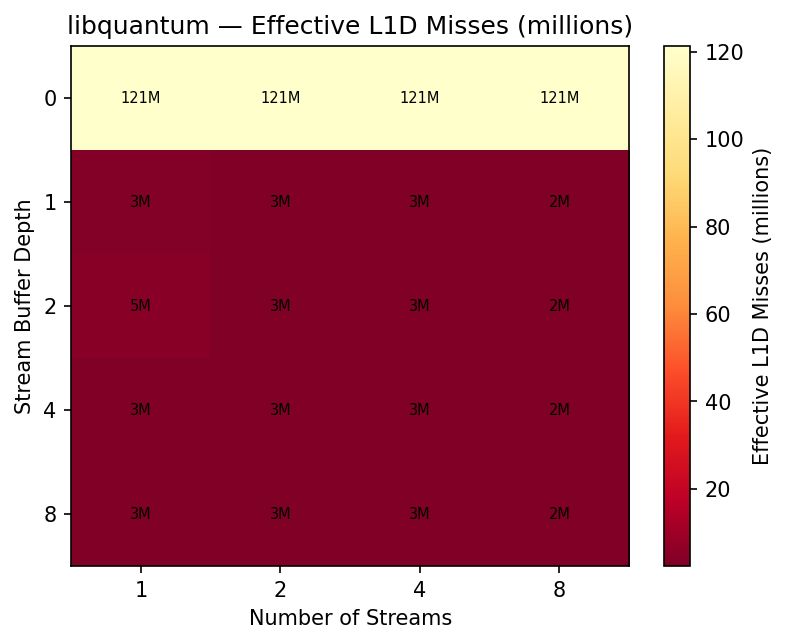
\includegraphics[width=\linewidth]{2d_libquantum_eff.png}
  \caption{\texttt{libquantum}}
\end{subfigure}
\hfill
\begin{subfigure}[b]{0.32\linewidth}
  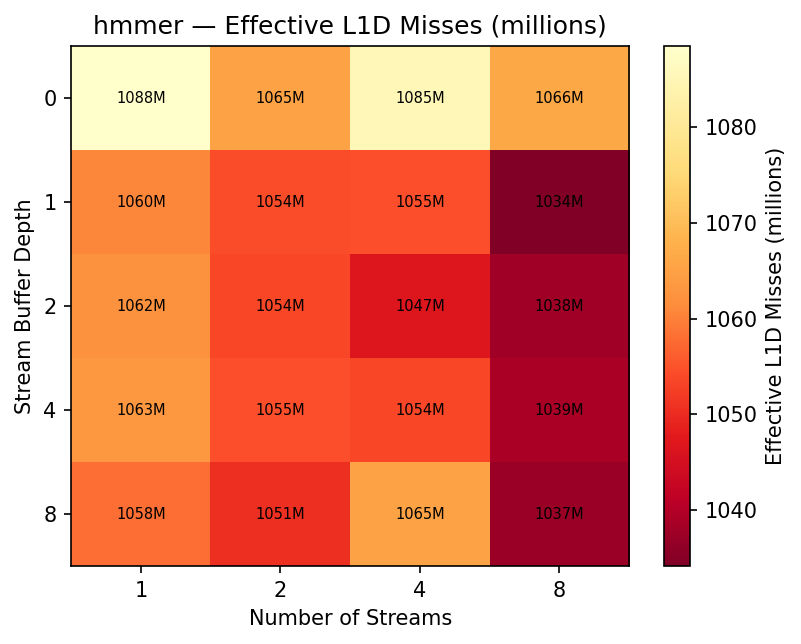
\includegraphics[width=\linewidth]{2d_hmmer_eff.png}
  \caption{\texttt{hmmer}}
\end{subfigure}
\hfill
\begin{subfigure}[b]{0.32\linewidth}
  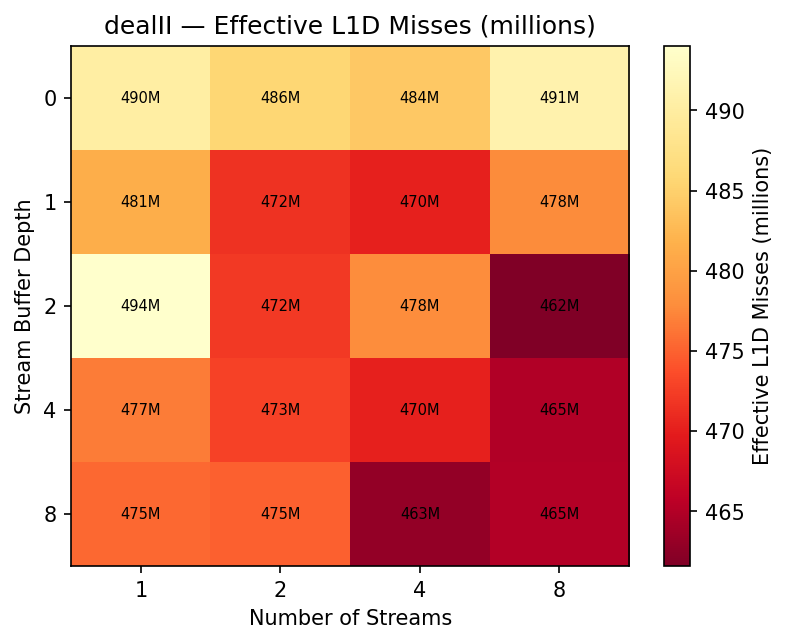
\includegraphics[width=\linewidth]{2d_dealII_eff.png}
  \caption{\texttt{dealII}}
\end{subfigure}
\caption{Effective L1D misses (millions) across all depth $\times$ stream
combinations (direct-mapped L1D). Darker red = fewer misses (better). For
\texttt{libquantum} any $D \geq 1$ saturates; for \texttt{hmmer} the buffer
is ineffective regardless of configuration; for \texttt{dealII} higher $N$
outweighs higher $D$.}
\label{fig:heatmaps}
\end{figure}

%─────────────────────────────────────────────────────────────────────────────
\section{Discussion and Conclusions}
%─────────────────────────────────────────────────────────────────────────────

\paragraph{Are the results expected?} Yes. The outcomes align precisely with
theoretical predictions for Jouppi-style stream buffers.

\textbf{The stream buffer is highly effective for libquantum.} A 97.7\%
reduction in effective L1D misses at the minimum depth demonstrates that the
workload's access pattern---long sequential scans over large arrays exceeding
the L1D capacity---is exactly what stream buffers are designed to exploit.
Saturation at $D=1$ indicates that a single prefetch line is enough to hide
the L2 latency for sequential accesses, an important design insight: deeper
buffers waste hardware resources and L2 bandwidth without further benefit for
this workload.

\textbf{The stream buffer is counter-productive for hmmer.} Although effective
misses drop by only 2.5\%, L2 bandwidth explodes nearly 9$\times$ at $D=8$.
A real system would experience L2 and memory bus saturation, likely degrading
performance despite the small miss-count improvement. The correct strategy for
\texttt{hmmer} is increased associativity (an 85\% miss reduction) rather than
prefetching.

\textbf{dealII occupies a middle ground.} Its mixed sequential-irregular access
pattern yields small but real prefetch benefits ($\sim$6\% at best) with
proportional L2 bandwidth costs. The most cost-efficient operating point is
$D=1$, $N=4$--8, which captures most of the benefit without the severe
bandwidth waste seen at higher depths.

\paragraph{Design Implications.}
These results underscore two fundamental principles of hardware prefetching.
First, \emph{coverage} depends on matching the prefetch strategy to the access
pattern: stream buffers excel at sequential access but are blind to irregular
patterns. Second, \emph{bandwidth} is a finite resource: prefetchers that
generate many useless requests pollute the memory hierarchy even when they do
not increase demand-miss latency directly.

In a practical design, stream buffers are best paired with a prefetch throttle
or confidence filter that monitors the hit rate and disables prefetching when
the ratio of hits to allocations is low. For a workload like \texttt{hmmer},
such a throttle would shut down the stream buffer almost immediately, avoiding
the bandwidth explosion while adding negligible area overhead.

\paragraph{Summary.}
A Jouppi stream buffer with $D=1$ and $N=1$ achieves a 97.7\% L1D miss
reduction for \texttt{libquantum} at negligible L2 bandwidth overhead, and is
essentially ineffective for \texttt{hmmer} and \texttt{dealII}. Increasing
depth or stream count beyond the minimum saturates benefit for sequential
workloads while linearly amplifying bandwidth consumption for irregular ones.
The associativity sweep confirms that conflict-miss-heavy workloads like
\texttt{hmmer} are better served by associativity than by prefetching.

\begin{thebibliography}{1}
\bibitem{jouppi1990improving}
Norman P. Jouppi.
\newblock Improving direct-mapped cache performance by the addition of a small
fully-associative cache and prefetch buffers.
\newblock In \emph{Proceedings of the 17th Annual International Symposium on
Computer Architecture (ISCA)}, pages 364--373, 1990.
\end{thebibliography}

\end{document}
